
\begin{figure}[h]
\vspace{-3mm}
    \centering
    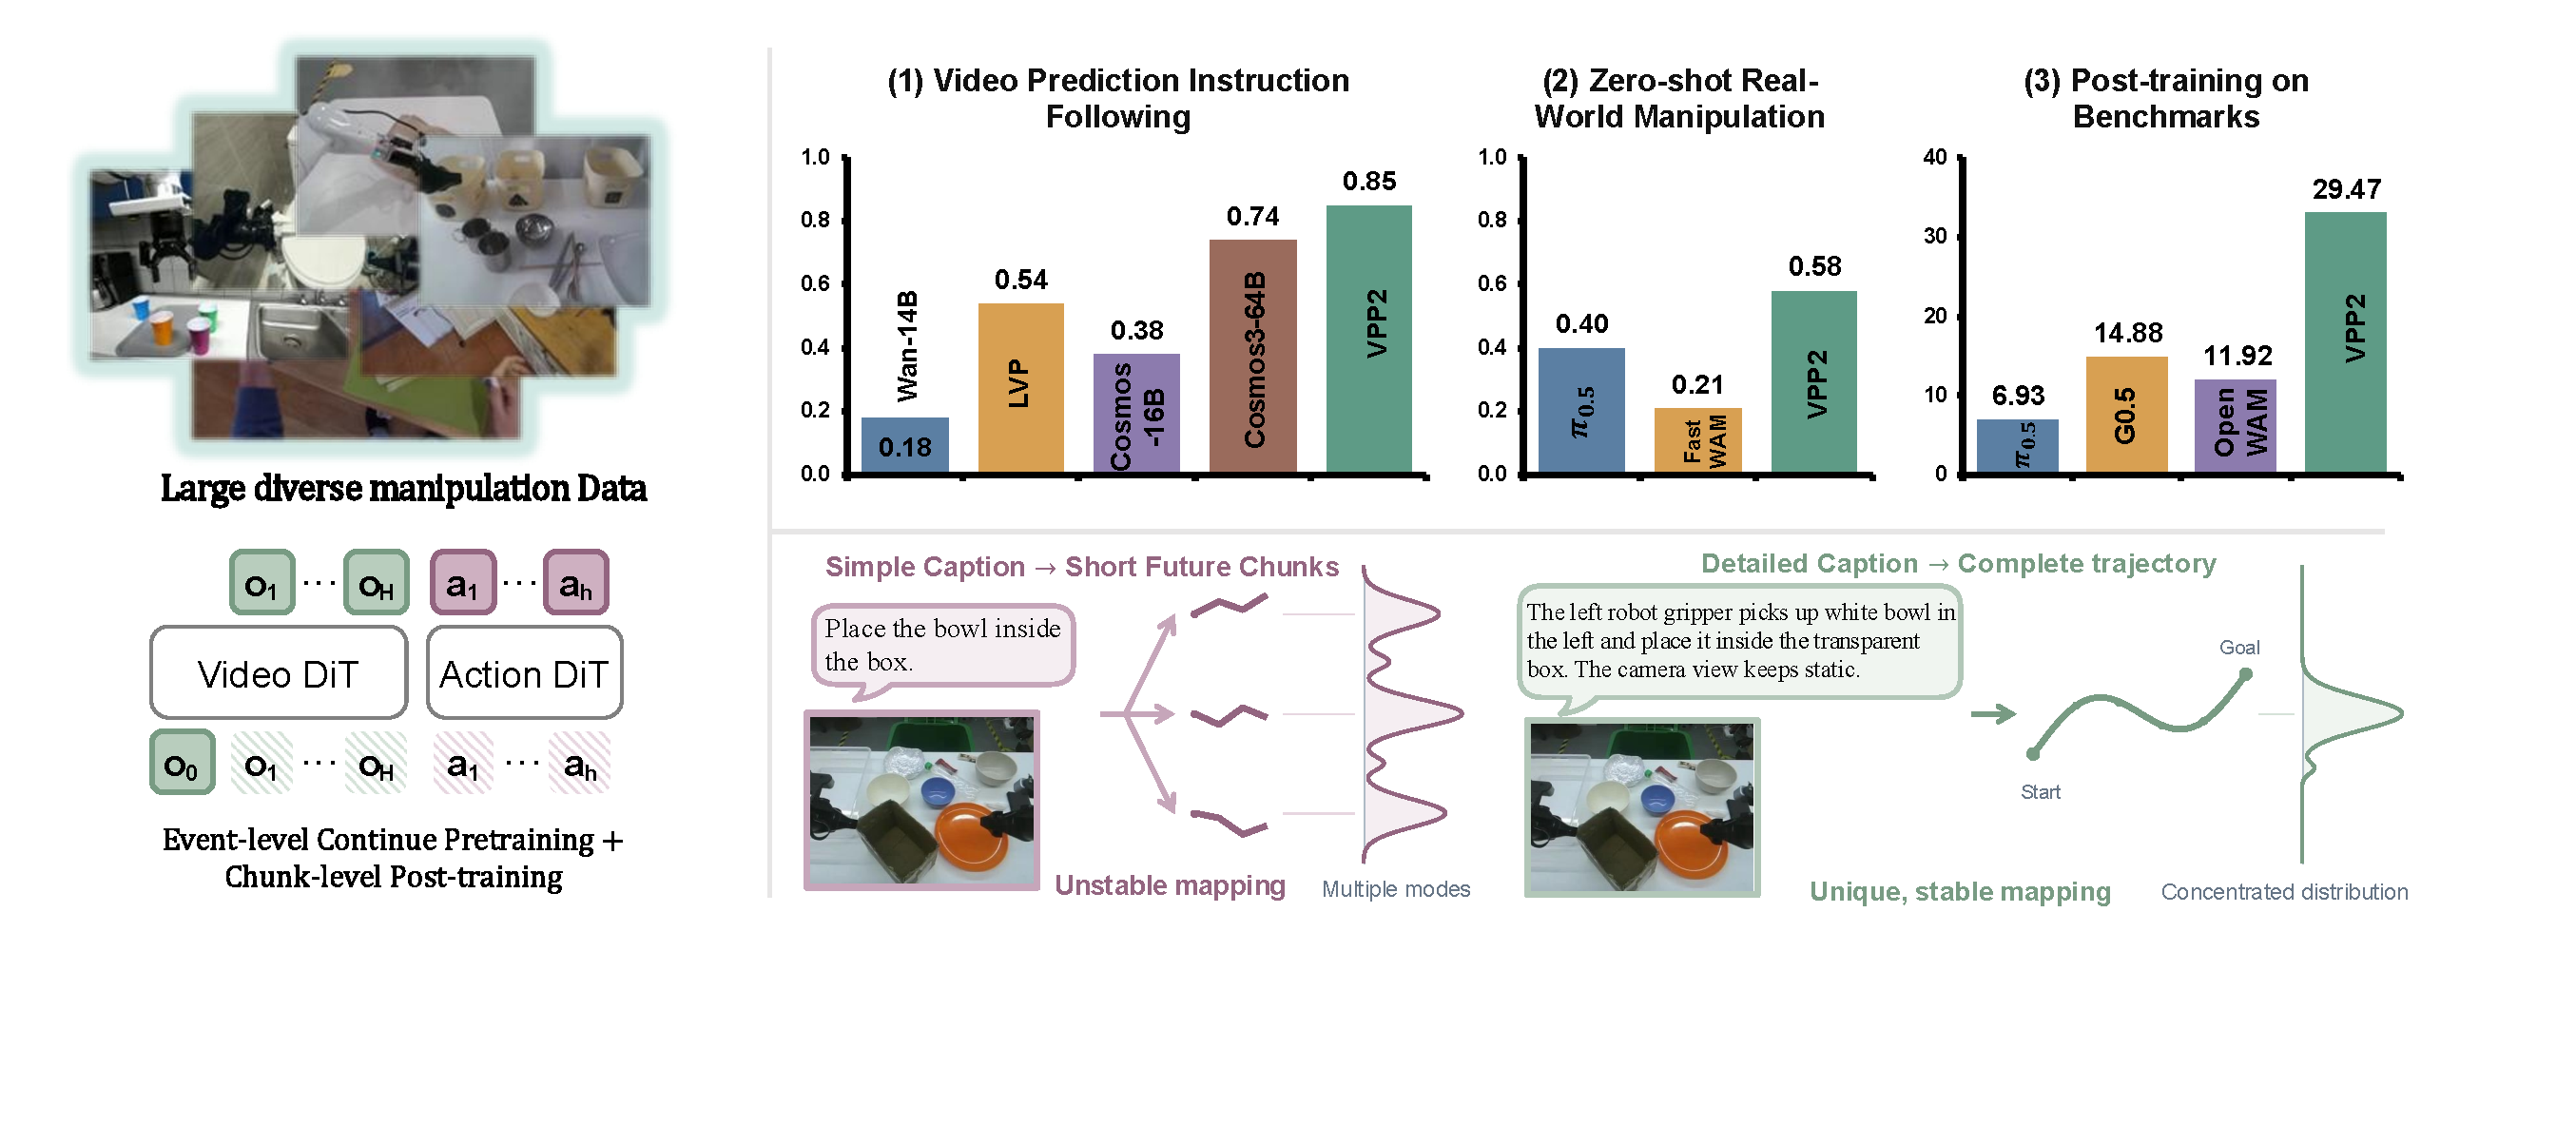
\includegraphics[width=1.0\linewidth]{figures/fig1_0926_scientific_colors_checked.pdf}
    \caption{A typical robot policy maps a simple instruction and an observation into a short action chunk. As datasets scale, this mapping becomes increasingly multimodal and uncertain, leading models to learn spurious short-horizon correlations. VPP2 first establishes consistent semantic-to-trajectory mappings via \textit{next event video prediction} with detailed captions, then post-trains and distills the model to generate short action chunks.}
    \label{fig:fig1}
    \vspace{-5mm}
\end{figure}

\section{Introduction}
\vspace{-2mm}
% World action models (WAMs) have emerged as an important class of generalist robot policies~\citep{hu2024video,liao2025genie,kim2026cosmospolicy,yuan2026fastwam,ma2026dit4dit}. 
% By building on video foundation models pretrained on internet-scale data~\citep{wan2025wan,agarwal2025cosmos}, WAMs use video prediction priors to guide action learning, with the promise of transferring the rich physical and semantic knowledge of video models into generalizable robot control.

World action models (WAMs) are developing rapidly and have become an important class of generalist robot policies~\citep{hu2024video,liao2025genie,kim2026cosmospolicy,yuan2026fastwam,ma2026dit4dit,li2026lingbotva,li2026wallwm,agibot2026geact2,ye2026dreamzero}. Many WAMs build on video foundation models~\citep{wan2025wan,agarwal2025cosmos,yang2025cogvideox}, aiming to transfer their rich priors about physical dynamics to policy learning. This premise is compelling: accurate, instruction-conditioned video predictions can guide action generation through an explicit or implicit inverse dynamics model~\citep{du2024learning,hu2024video}. However, prior work~\citep{zhang2026qwen} has found that existing WAMs often perform well only on a narrow set of seen tasks, while producing unreliable future motion predictions in unseen, out-of-distribution scenarios. These prediction failures, in turn, lead to erroneous actions. In recent benchmarks that require generalization, robot policies, including WAMs, with near-perfect success rates on standard evaluation suites suffer substantial performance drops under perturbed task configurations and novel skill compositions~\citep{zhou2025liberopro,li2025vlas,mishra2026understanding}.

% We identify two key factors that lead to the weakness of WAMs: First, base video models are optimized for general-purpose content creation rather than manipulation, and therefore often fail to follow manipulation instructions faithfully. Second, after WAMs introduce additional action components or leaning target to pretrained-video foundation models, the generalization of the video models are largely demaged.

We identify two key factors that limit the generalization of existing WAMs to unseen scenarios. First, base video models are primarily optimized for creative content generation and aesthetic quality rather than precise physical dynamics, and therefore often fail to follow manipulation instructions faithfully~\citep{chen2025large,zhang2026qwen}. Second, introducing action-specific components or training objectives into pretrained video foundation models can substantially degrade their generalization capabilities~\citep{mishra2026understanding}.

To address these issues, we introduce Video Prediction Policy 2 (VPP2), a WAM that achieves strong zero-shot generalization in both video prediction and action generation. Our first objective is to train a generalizable video foundation that can faithfully follow instructions and make future predictions grounded in the current observation, without unsupported changes to the scene or task. To this end, we annotate each clip with a detailed caption specifying the manipulation process, active end effector, and target object, and perform \textit{event-level} video prediction training. As illustrated in Figure~\ref{fig:fig1}, detailed captions and complete event-level trajectory prediction substantially reduce uncertainty in future prediction and encourage consistent mappings from semantic descriptions to visual trajectories, improving generalization across diverse instructions. We then post-train the video model to predict fixed-horizon future chunks and apply consistency distillation~\citep{song2023consistency} to obtain a single-step visual planner for real-time robot execution. Finally, we introduce an action expert through a mixture-of-transformers (MoT) architecture~\citep{liang2025mixture} to learn an implicit inverse dynamics model conditioned on the predicted future. During policy execution, we pair VPP2 with a VLM planner~\citep{bai2025qwen3,seed2026seed2} that translates open-ended instructions into explicit subtask instructions.

Our experiments demonstrate three key advantages of VPP2. (1) VPP2-14B follows manipulation instructions faithfully, outperforming Cosmos3-64B~\citep{agarwal2026cosmos} by 11\% in instruction-following success rate on open-ended tasks. (2) VPP2 exhibits strong zero-shot manipulation capabilities on a real-world ALOHA platform~\citep{zhao2023learning}, achieving an average success rate of 58.5\% across 10 task categories, compared with 40.0\% for $\pi_{0.5}$~\citep{intelligence2025pi_} and 20.5\% for Fast-WAM~\citep{yuan2026fastwam}. (3) Following benchmark-specific post-training, VPP2 achieves the highest success rates among evaluated methods on LIBERO-Pro~\citep{zhou2025liberopro} (45.0\%, compared with 11.0\% for the strongest baseline), LIBERO-OOD~\citep{li2025vlas,mishra2026understanding} (63.9\%), and RoboDojo~\citep{chen2026robodojo} (32.26\%, state-of-the-art).

% the post-training on video model WAMs typically train video prediction on short, chunk-level clips with terse instructions, and naively incorporating action learning pulls the video model toward the same ambiguous short-horizon mapping, substantially degrading its generalization.
% We attribute this limitation to the uncertainty of the learning target. As illustrated in Figure~\ref{fig:fig1}, a typical robot policy maps a simple instruction and an observation to a short action chunk. As datasets scale in size and diversity, this mapping becomes increasingly multi-modal and ambiguous, leading models to learn spurious short-horizon correlations rather than grounding actions in the instruction. Existing WAMs inherit this issue in two ways. 

% To address these issues, we introduce Video Prediction Policy 2 (VPP2), a WAM that achieves strong zero-shot generalization in both video prediction and action generation. Our central insight is that reducing uncertainty in future prediction is key to generalization across manipulation tasks. First, we curate a large-scale, diverse dataset of robot, human, and general manipulation videos, annotate each clip with a detailed caption that specifies the manipulation process, the active end effector, and the target object, and perform \textit{event-level} continued pretraining in which each sample covers a complete subtask. This establishes consistent mappings from semantic descriptions to future trajectories. Second, we post-train the video model to predict fixed-horizon future chunks and distill it into a single-step visual planner, enabling real-time inference. Finally, we introduce an action expert through a mixture-of-transformers (MoT) architecture that learns an implicit inverse dynamics model conditioned on the predicted future, and pair VPP2 with a VLM planner that converts open-ended instructions into explicit subtasks. The full policy generates an action chunk in approximately 0.22 seconds.



% In summary, our contributions are as follows:
% \begin{itemize}
%     \item We identify the uncertainty of short-horizon prediction targets as a key factor limiting the generalization of WAMs, and show that incorporating action learning naively degrades the generalization of video models.
%     \item We propose VPP2, which combines event-level video pretraining with detailed captions, fixed-horizon post-training with single-step distillation, and an MoT action expert, yielding a real-time policy with strong zero-shot generalization.
%     \item We demonstrate that better prediction leads to better action: VPP2 achieves state-of-the-art instruction following in video prediction, strong zero-shot real-world manipulation, and the highest success rates on challenging generalization benchmarks.
% \end{itemize}
